\documentclass[11pt]{article}
\usepackage[margin=2.2cm]{geometry}
\usepackage[T1]{fontenc}
\usepackage[utf8]{inputenc}
\usepackage{lmodern,microtype,amsmath,amssymb,booktabs,graphicx}
\usepackage[colorlinks=true,allcolors=blue!50!black]{hyperref}
\usepackage{xcolor}
\title{Seguimiento científico para OMS}
\author{Mathias Rodríguez Castro}
\date{17 de octubre de 2026}
\emergencystretch=1em
\begin{document}
\maketitle
\noindent Se cerraron cuatro estudios acotados: transferencia a otra aplicación,
trayectoria de factores, tolerancia entera y ciclo nativo completo. La conclusión
es una validación más amplia del procedimiento, con límites comprobados y sin
una tercera contribución matemática.

\section*{Transferencia aplicada y ejemplo en unidades originales}
Ocho horizontes prefijados del ejemplo Kondili de STN-Scheduler, independiente del
generador hidroeléctrico, producen 96 llamadas con tres semillas nuevas y cuatro
controles. Dos horizontes son anclas conocidas; seis son nuevos. Masa, lógica y
dinero tienen presupuestos declarados antes de resolver: $10^{-5}$ kg, $10^{-5}$ y
$10^{-3}$ unidades monetarias. Son objetivos numéricos, no estándares industriales.

\begin{center}
\begin{tabular}{lr}\toprule
Método diádico & Cumple todos los presupuestos\\\midrule
L2 &24/24\\ Budget-L2&24/24\\ L2-tight&24/24\\ L2-NF3&23/24\\\bottomrule
\end{tabular}
\end{center}

En H40, semilla 149, NF3 devuelve $W=0$ y $B=1.110407442\cdot10^{-4}$ kg
en $B-200W\le0$: 111.041 mg de violación frente al objetivo de 10 mg.
Los enteros son exactos. El factor L2 $2^{-8}$ da residuo exportado
$4.338\cdot10^{-7}<10^{-6}$. Budget elige $2^{-3}$: la cota condicional,
incluyendo redondeo entero, es $8.2$ mg. Sus puntos cumplen. L2 también cumple;
el hallazgo demuestra transferencia y trazabilidad, sin recuperación adicional
frente al control directo.

Ocho referencias NF3 y ocho LP de patrón fijado dejan un testigo exacto y siete
resultados desconocidos. Sólo 12 de los 96 contrastes de cotas tienen ese testigo;
los otros 84 quedan desconocidos. No se buscaron patrones alternativos. Los fallos
del LP exacto no son pruebas de inviabilidad del MILP.

\section*{Costo del ciclo C++ completo}
En 18 pares modelo/semilla, los modelos ordenados, puntos, endpoints y trabajo
nativo son idénticos. La razón geométrica de tiempo completo C++/Python es
\textbf{0.824}, un 17.6\% menos en este equipo. Ambos procesos incluyen startup,
generación una vez, metadata original, selección, exportación, importación/cotejos,
solve, verificación física y persistencia. Compilación y testigos previos son aparte.
No hubo otra campaña propia de solver en paralelo. La máquina es compartida y
los tiempos son descriptivos. La aceleración de preparación de 3.7--6.4 no se
extrapola al ciclo completo.

\begin{center}\small
\begin{tabular}{lrrr}
\toprule
Model & Python (s) & C++ (s) & C++/Python time\\
\midrule
001 & 4.378 & 3.974 & 0.908\\
005 & 1.636 & 1.218 & 0.744\\
022 & 1.620 & 1.184 & 0.731\\
027 & 2.874 & 2.472 & 0.860\\
031 & 1.586 & 1.185 & 0.747\\
046 & 10.555 & 10.416 & 0.987\\
All 18 pairs & -- & -- & 0.824\\
\bottomrule
\end{tabular}

\end{center}

\section*{Límite de robustez de la tolerancia entera}
Se mantienen modelos, semillas, presolve y demás parámetros; los factores del
contrato se recomputan coherentemente con la reserva entera. Se agregan 36 MILP y
18 abstenciones a las 54 llamadas reutilizadas. Los 12 testigos previos son
válidos para las mismas exportaciones; no se repiten LP.

\begin{center}\small
\resizebox{\linewidth}{!}{\begin{tabular}{rrrrrrr}
\toprule
IntFeasTol & $\delta_V$ & Calls & Abstentions & Budgets & B/G & $W/W_{\rm NF3}$\\
\midrule
$10^{-9}$ & 30 & 18/18 & 0 & 18/18 & 0/0 & 0.411\\
$10^{-9}$ & 100 & 18/18 & 0 & 18/18 & 0/0 & 0.362\\
$2^{-28}$ & 30 & 0/18 & 18 & -- & -- & --\\
$2^{-28}$ & 100 & 18/18 & 0 & 18/18 & 1/0 & 0.356\\
\bottomrule
\end{tabular}
}
\end{center}

A $2^{-28}$, la reserva entera agota 30 m$^3$ en los seis modelos. La abstención
no implica inviabilidad. A 100 m$^3$ se conserva el cumplimiento y menor trabajo,
pero una cota sigue contradicha. El régimen sin contradicciones detectadas no es
robusto a estos dos valores y no certifica optimalidad.

\section*{Qué explica el análisis por fila}
Entre los objetivos ensayados de 30 a 1,000 m$^3$ cambia el mismo conjunto de
8,640 factores, exclusivamente de activación. Sus magnitudes disminuyen.
Con $R_i$ como reserva combinada, la inspección directa verifica
\[
\alpha_i=\operatorname{ceil}_{64}\max\{10^{-9},\epsilon/(\delta_V-R_i)\}.
\]
Los umbrales que vuelven admisible L2 están entre 1,008.779 y 1,013.068 m$^3$.
Se comprobaron 53,280 factores compatibles, 7,200 intervalos incompatibles y
319,680 filas no activación sin cambios, sin importar el selector ni el runner.
Los puntos automáticos cumplen la hipótesis exportada, incluso con cotas
contradichas. Esto localiza la representación cambiada; no identifica cuál
operación interna del solver causa el comportamiento. La banda favorable resume
dos objetivos ensayados, no todos los valores intermedios.

\section*{Protocolo, preservación y alcance editorial}
Total nuevo: 176 MILP y ocho intentos LP. Se conservan resultados adversos,
abstenciones, siete refinamientos desconocidos y el fallo de preflight por orden
de construcción de la fuente STN, anterior a optimizar. La corrección verifica
el multiconjunto matemático de filas y restaura el orden ya congelado. Ningún
resultado adverso se reejecutó ni se modificó el generador original.

El paper conserva dos contribuciones. Aporta la validación externa con su control
L2 positivo y la medición de software; declara la falta de robustez de tolerancia.
El escalado conjunto, DW y cortes permanecen fuera. El autor confirmó que CAP no
apoyó este trabajo. Se reduce el abstract por precaución; el límite oficial no
pudo verificarse por HTTP 403. DOI y publicación permanecen diferidos.

Los programas y resultados están en \texttt{RESULTADOS.md}. Los checkers no
optimizan; usan Python, NumPy y HiGHS 1.15.1 sólo como lector. El artefacto completo
incluye las dependencias archivadas y las fuentes MIT de STN-Scheduler.

\clearpage
\begin{figure}[p]\centering
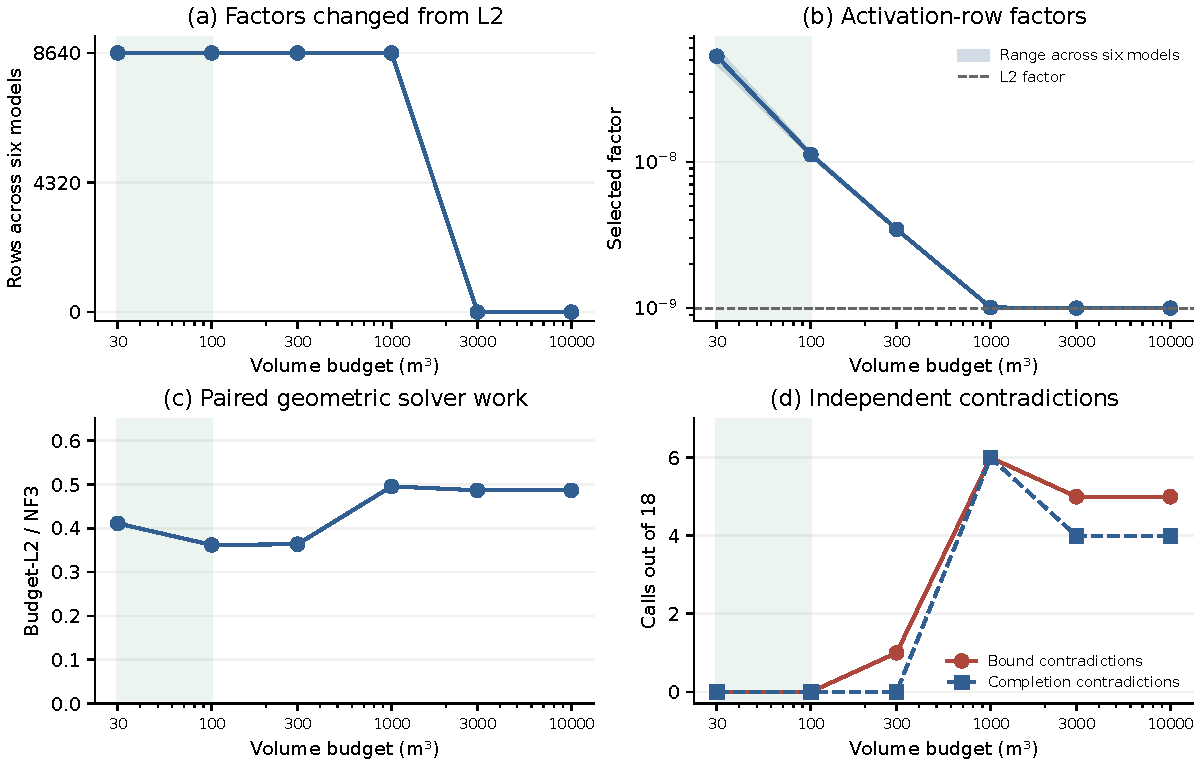
\includegraphics[width=\linewidth]{mechanism/precision-transition.pdf}
\caption{Trayectoria de factores y resultados existentes con presolve automático,
seis modelos y tres semillas. Se muestran todos los presupuestos compatibles
en los seis casos. El cambio en número de filas no explica la transición entre
30 y 1,000 m$^3$; las magnitudes cambian. Menor esfuerzo y ausencia de flags no
constituyen certificación global. La franja sombreada corresponde a los dos
objetivos observados favorables. No hubo nuevas llamadas para esta figura.}
\end{figure}
\end{document}
